\documentclass[a4paper,12pt]{article}
\usepackage[a4paper, portrait, margin=0.8in]{geometry}
\usepackage{graphicx} 
\usepackage{caption}
\usepackage{subcaption} 
\usepackage{float}
\usepackage{tikz}
\usepackage{xparse}
\usepackage{xstring}
\usepackage{karnaugh-map}

\def\changemargin#1#2{\list{}{\rightmargin#2\leftmargin#1}\item[]}
\let\endchangemargin=\endlist 

\begin{document}
\pagenumbering{gobble}
\title{CEG2136 LAB 2 \\\ Group 21}
\author{Ryan Fleck - 8276723 \\\ Xiuzhu Li - 8571645}
\maketitle
\newpage
\pagenumbering{roman}
\tableofcontents
\listoffigures
\newpage
\pagenumbering{arabic}  


\section{Theoretical Implementation}

\subsection{Lab Objectives}
This second lab continues to introduce students to the basic components of digital systems, namely JK flip flops and essential logical elements. Students will use \textit{Altera Quartus II} to design, compile and run/verify two different sequential circuits.
\begin{enumerate}
\item From a given sequence, karnaugh maps and input equations for the JKs will be derived.
\item In \textit{Altera Quartus II}, the JKs will be connected according to the derivations.
\item The counters will be tested using a push-button and a free-running clock that will be read using an oscilloscope.
\end{enumerate}

\subsection{Discussion of Requirements}
The goal of the lab is to implement a '3 bit synchronous modulo 6' and '4 bit synchronous BCD' counters and have them run without errors on the \textit{Altera DE2-115 FPGA}, with every set of inputs resulting in the output predicted by their karnaugh map. These two counters will be tested using one of two possible methods, either visualizing the output on an oscilloscope \ref{fig:Scope} or manually with a push-button and LEDs on the \textit{Altera DE2-115 FPGA}.


Required equipment and items:
\begin{enumerate}
\item An x86-compatible PC running \textit{Quartus II}.
\item The \textit{Altera DE2-115 FPGA}.
\item CEG2136 lab manual.
\item Oscilloscope and required interface.
\end{enumerate}

\subsection{Proposed Algorithmic Solution}


\subsubsection{Karnaugh Maps for Counter A}
\begin{center}

\begin{figure}[H]
\begin{tabular}{cc}

\begin{karnaugh-map}[4][2][1][$Q_1Q_0$][$Q_2$][J0]
\minterms{6}
\maxterms{0,2,4}
\autoterms[X]
\implicant{7}{6}
\end{karnaugh-map}
&
\begin{karnaugh-map}[4][2][1][$Q_1Q_0$][$Q_2$][J0]
\minterms{5}
\maxterms{3}
\autoterms[X]
\implicant{4}{6}
\end{karnaugh-map}
\\
\large $J_0$ = $Q_2Q_1$
&
\large $K_0$ = $Q_2$

\end{tabular}
\caption{Karnaugh Maps for A-$JK_0$}
\label{fig:AJK0}
\end{figure}



\begin{figure}[H]
\begin{tabular}{cc}

\begin{karnaugh-map}[4][2][1][$Q_1Q_0$][$Q_2$][J0]
\minterms{0}
\maxterms{4,5}
\autoterms[X]
\implicant{0}{2}
\end{karnaugh-map}
&
\begin{karnaugh-map}[4][2][1][$Q_1Q_0$][$Q_2$][J0]
\minterms{3}
\maxterms{2,6}
\autoterms[X]
\implicant{1}{7}
\end{karnaugh-map}
\\
\large $J_1$ = $Q_2'$
&
\large $K_1$ = $Q_0$

\end{tabular}
\caption{Karnaugh Maps for A-$JK_1$}
\label{fig:AJK1}
\end{figure}



\begin{figure}[H]
\begin{tabular}{cc}

\begin{karnaugh-map}[4][2][1][$Q_1Q_0$][$Q_2$][J0]
\minterms{2,3}
\maxterms{0}
\autoterms[X]
\implicant{3}{6}
\end{karnaugh-map}
&
\begin{karnaugh-map}[4][2][1][$Q_1Q_0$][$Q_2$][J0]
\minterms{4,6}
\maxterms{5}
\autoterms[X]
\implicant{0}{4}
\implicant{2}{6}
\end{karnaugh-map}
\\
\large $J_2$ = $Q_1$
&
\large $K_2$ = $Q_0'$

\end{tabular}
\caption{Karnaugh Maps for A-$JK_2$}
\label{fig:AJK2}
\end{figure}
\end{center}




\subsubsection{Karnaugh Maps for Counter B}
\begin{figure}[H]
\begin{tabular}{cc}

\begin{karnaugh-map}[4][4][1][$Q_1Q_0$][$Q_3Q_2$][J0]
\minterms{0,2,4,6,8}
\maxterms{}
\autoterms[X]
\implicant{0}{10}
\end{karnaugh-map}
&
\begin{karnaugh-map}[4][4][1][$Q_1Q_0$][$Q_3Q_2$][J0]
\minterms{1,3,5,7,9}
\maxterms{}
\autoterms[X]
\implicant{0}{10}
\end{karnaugh-map}
\\
\large $J_0$ = 1
&
\large $K_0$ = 1

\end{tabular}
\caption{Karnaugh Maps for B-$JK_0$}
\label{fig:JK0}
\end{figure}


\begin{figure}[H]
\begin{tabular}{cc}

\begin{karnaugh-map}[4][4][1][$Q_1Q_0$][$Q_3Q_2$][J0]
\minterms{1,5}
\maxterms{0,4,8,9}
\autoterms[X]
\implicant{1}{7}
\end{karnaugh-map}
&
\begin{karnaugh-map}[4][4][1][$Q_1Q_0$][$Q_3Q_2$][J0]
\minterms{3,7}
\maxterms{2,6}
\autoterms[X]
\implicant{1}{11}
\end{karnaugh-map}
\\
\large $J_1$ = $Q_3'Q_0$
&
\large $K_1$ = $Q_0$

\end{tabular}
\caption{Karnaugh Maps for B-$JK_1$}
\label{fig:JK1}
\end{figure}



\begin{figure}[H]
\begin{tabular}{cc}

\begin{karnaugh-map}[4][4][1][$Q_1Q_0$][$Q_3Q_2$][J0]
\minterms{3}
\maxterms{0,1,2,8,9}
\autoterms[X]
\implicant{3}{11}
\end{karnaugh-map}
&
\begin{karnaugh-map}[4][4][1][$Q_1Q_0$][$Q_3Q_2$][J0]
\minterms{7}
\maxterms{4,5,6}
\autoterms[X]
\implicant{3}{11}
\end{karnaugh-map}
\\
\large $J_2$ = $Q_0Q_1$
&
\large $K_2$ = $Q_0Q_1$

\end{tabular}
\caption{Karnaugh Maps for B-$JK_2$}
\label{fig:JK2}
\end{figure}



\begin{figure}[H]
\begin{tabular}{cc}

\begin{karnaugh-map}[4][4][1][$Q_1Q_0$][$Q_3Q_2$][J0]
\minterms{7}
\maxterms{0,1,2,3,4,5,6}
\autoterms[X]
\implicant{7}{15}
\end{karnaugh-map}
&
\begin{karnaugh-map}[4][4][1][$Q_1Q_0$][$Q_3Q_2$][J0]
\minterms{9}
\maxterms{8}
\autoterms[X]
\implicant{1}{11}
\end{karnaugh-map}
\\
\large $J_3$ = $Q_2Q_1Q_0$
&
\large $K_3$ = $Q_0$

\end{tabular}
\caption{Karnaugh Maps for B-$JK_3$}
\label{fig:JK3}
\end{figure}



\section{Design}

\subsection{QUARTUS II Circuit Diagrams}

The circuits were implemented in \textit{Altera Quartus II} using components chosen by reading the Karnaugh maps from \textit{Figure \ref{fig:AJK0}} through  to \textit{Figure \ref{fig:JK3}}.

\begin{figure}[H]
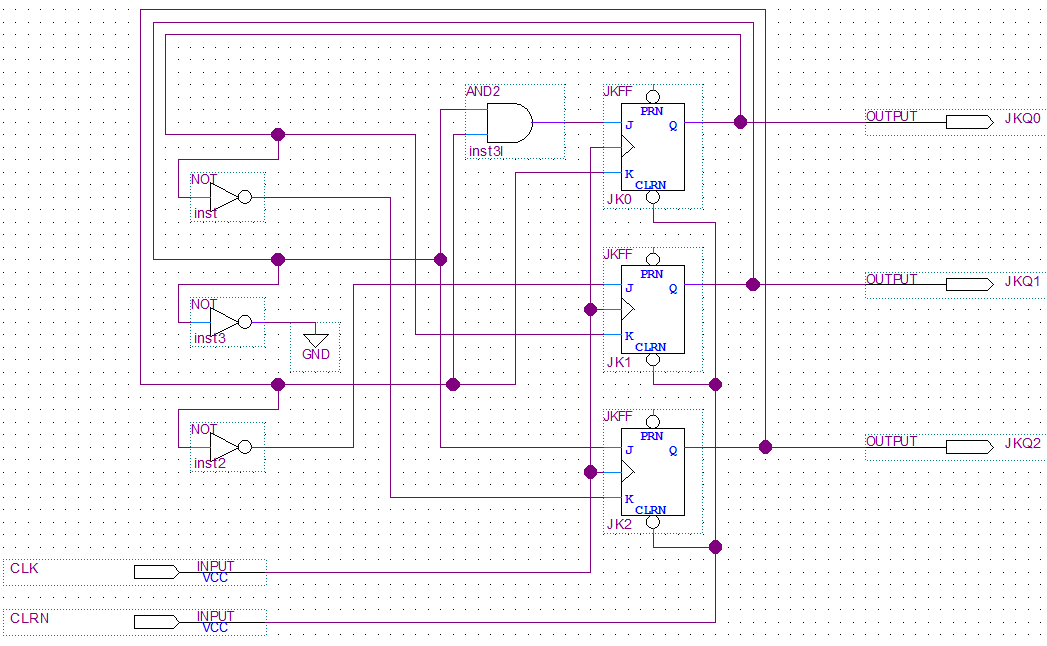
\includegraphics[width=\textwidth]{Images/LAB2_CircuitA.PNG} 
\caption{Circuit 'A', a 3-bit counter.}
\label{fig:CircA}
\end{figure}

\begin{figure}[H]
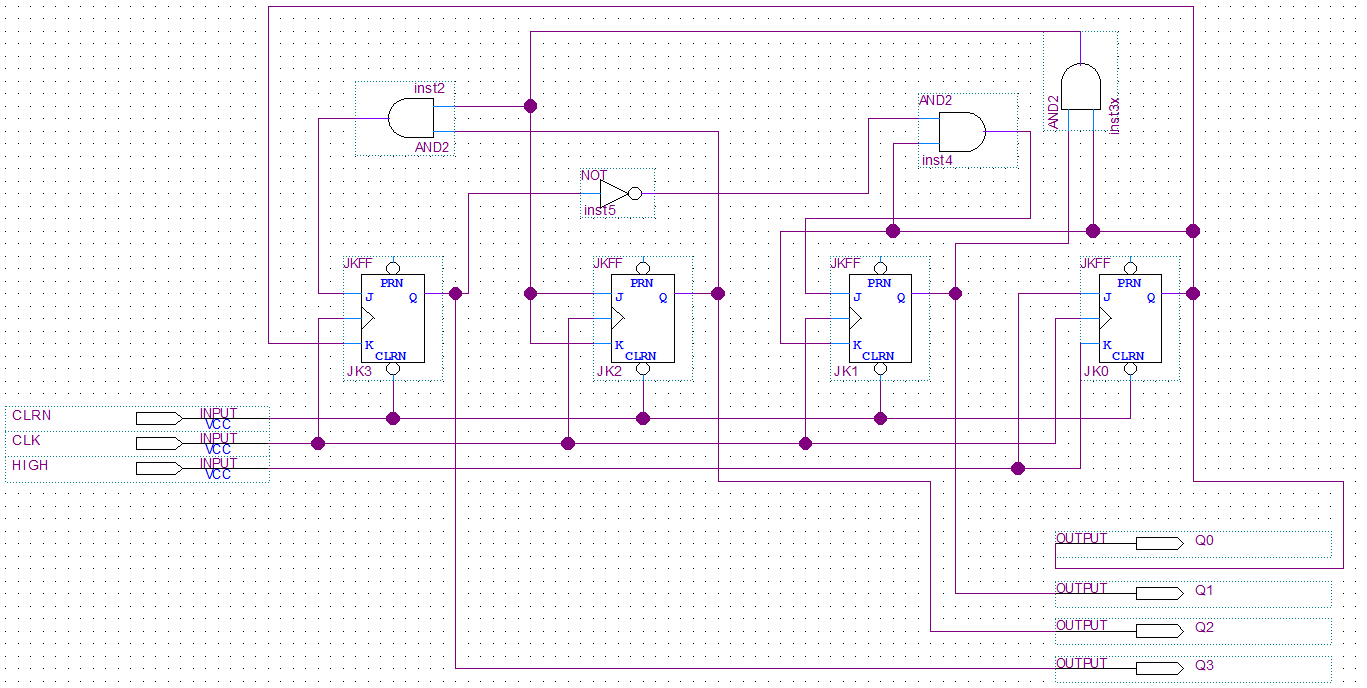
\includegraphics[width=\textwidth]{Images/LAB2_CircuitB.PNG} 
\caption{Circuit 'B', a 4-bit counter.}
\label{fig:CircB}
\end{figure}


\subsection{Components Utilized}

Our designs, as shown in as shown in \textbf{Figure \ref{fig:CircA}} and \textbf{Figure \ref{fig:CircB}}, were implemented as intended with simple AND,OR and NOT logic gates and JK Flipflops. No alternative components, that is, similar components with different part numbers (than those specified in the lab manual,) were used to create the logical circuit.

\subsection{Implemented Solution}
When implementing our solution, we took the following steps:
\begin{enumerate}
\item \textit{Altera Quartus II} was opened and the file was initialized.
\item Both circuits were implemented according to the karnaugh maps.
\item Pins were added and assigned correctly.
\item The file was compiled.
\item At this point, the circuits were ready to simulate/verify/apply test procedures.
\end{enumerate}
\subsection{Challenging Problems Encountered}
No major problems were encountered in this section of the lab. However, we did rush this portion of the lab, as we failed to fully complete the karnaugh maps for the 4-bit BCD counter in time for the lab. Our only major hangups were encountered 




\section{Implementation}

\subsection{Simulation Results}
\textbf{Figure \ref{fig:WavA}} \textbf{Figure \ref{fig:WavB}} both show a set of 16 clock cycles, enough to fully visualize a single full run of a 4-bit sequential counter and two 8-step runs of a generic 3-bit sequential counter. Both simulated cycles ran as expected, and we didn't encounter any errors in this part of our testing.

\subsection{Block Diagrams}

\begin{figure}[H]
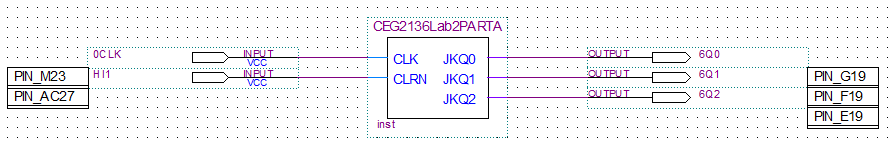
\includegraphics[width=\textwidth]{Images/LAB2_TestA.PNG} 
\caption{Block Diagram for Circuit A}
\label{fig:BlockDiagA}
\end{figure}

\begin{figure}[H]
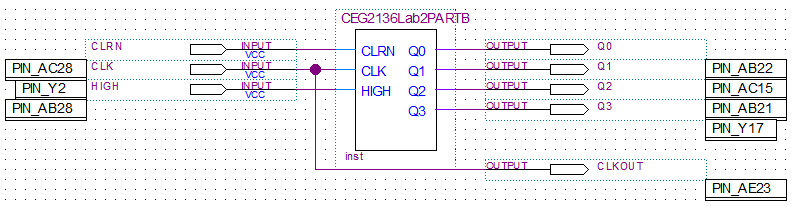
\includegraphics[width=\textwidth]{Images/LAB2_TestB.PNG} 
\caption{Block Diagram for Circuit B}
\label{fig:BlockDiagB}
\end{figure}


\subsection{Simulated Waveforms}

\begin{figure}[H]
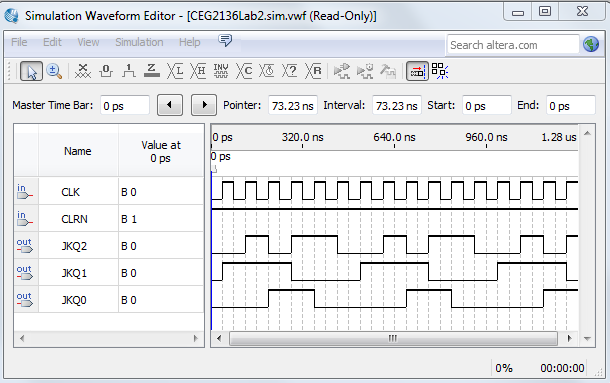
\includegraphics[width=\textwidth]{Images/LAB2_WaveFormA.PNG} 
\caption{Logical Circuit Waveform Output for Circuit A}
\label{fig:WavA}
\end{figure}

\begin{figure}[H]
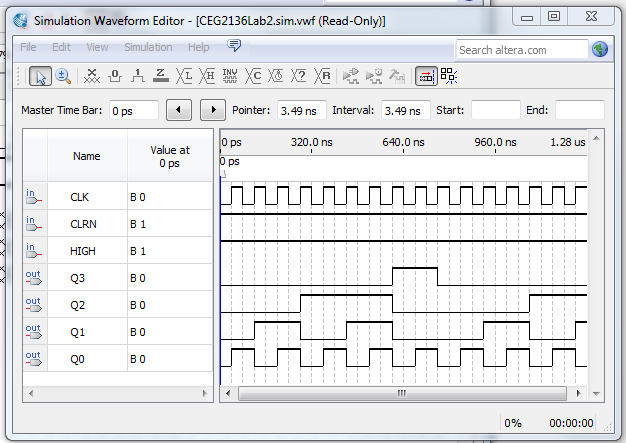
\includegraphics[width=\textwidth]{Images/LAB2_WaveFormB.PNG} 
\caption{Logical Circuit Waveform Output for Circuit B}
\label{fig:WavB}
\end{figure}

\subsection{Oscilloscope Output}

\begin{figure}[H]
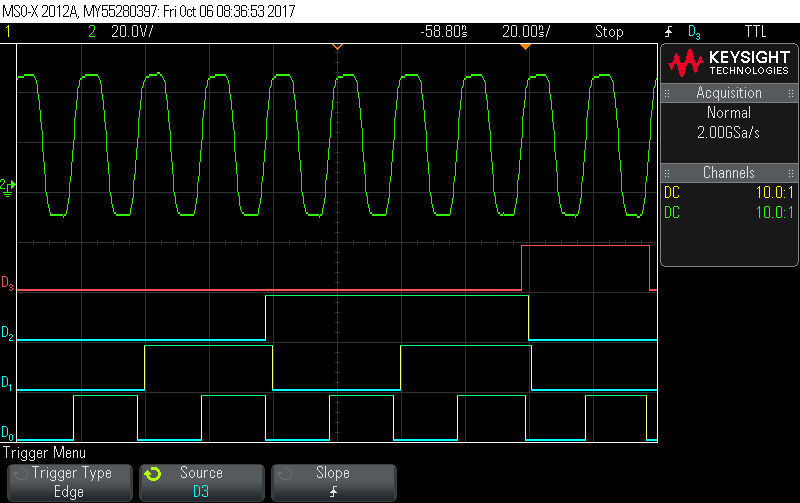
\includegraphics[width=\textwidth]{Images/scope_4.png} 
\caption{Oscilloscope Output from 4-Bit Synchronous BCD Counter}
\label{fig:Scope}
\end{figure}


\section{Discussion}
After exhaustive testing of our running logical circuit, we simulated the BCD counter using \textit{Altera DE2-115 FPGA} and, by connecting \textit{GPIO 40-pin assignments}, we managed to output the counter signal to Oscilloscope, while the clock frequency was transfered by the coaxial cable. The dynamic images we got from Oscilloscope' screen (See \textbf{Figure \ref{fig:Scope}}) was perfect and precise, showing the exactly how the BCD counter would work. After we had done with Oscilloscope experiment, we began our simulation of the 3-bit counter with the 'push-button' method, in which we assigned the CLK pin from the modulo 6 counter to a button switch on the \textit{Altera DE2-115 FPGA} board. In this case, each time of push-and-release to the button acted as a clock cycle, going from 0 to 1 then back to 0. After LED pins were assigned for the three digits as well as compilation done, we can advance the cycle manually by pressing the button switch. Each press and release advanced the 3-bit counter by one clock period and we could observe the state of the simulated counter via the Altera board's LED outputs.



\subsection{Errors Encountered}
\textbf{Figure \ref{fig:Uploaded}} shows our final pin plan. This is where we had the most difficulty - At one point, our lab group had the oscilloscope up and running, but didn't have any output. After checking the pin planner again, we found that it simply hadn't saved the assignments at all.
\begin{figure}[H]
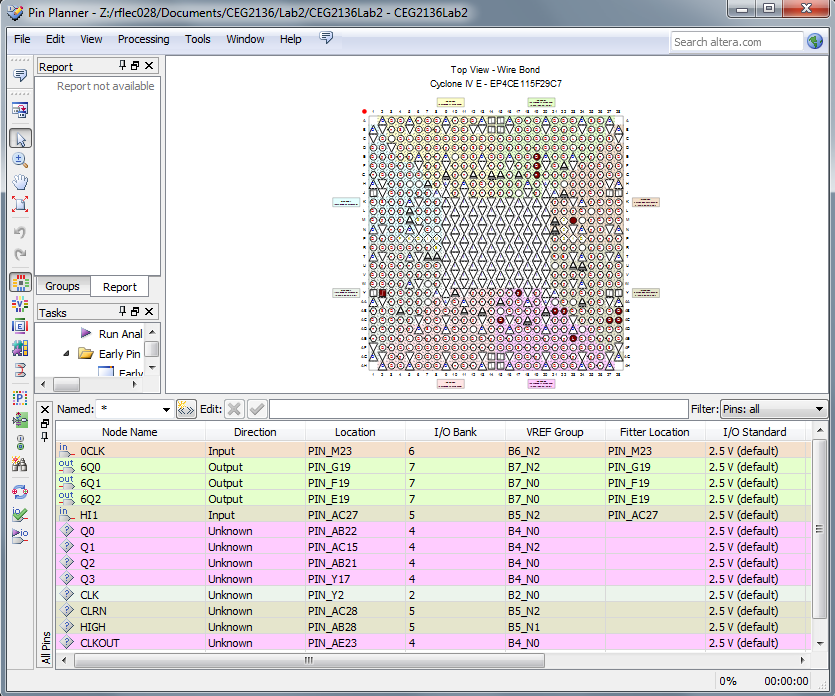
\includegraphics[width=\textwidth]{Images/LAB2_PinAssignment.PNG} 
\caption{Implemented Pin Plan for EP4CE115F29 Device.}
\label{fig:Uploaded}
\end{figure}


\subsection{Conclusions}
During lab 2 we continued to experiment with sequential circuits, and learned how to use Oscilloscope kit to visualize their outputs. The oscilloscope was new content introduced to this course, so was our first time contacting with such expensive equipment. It seems using Oscilloscope to simply be a real-time waveform simulator is a over-kill, but we expect further discovery on it, along with more complex course content we will encounter. Lab 2 emphasized on the structure and functionality of sequential circuits, and by utilizing K-maps and various lab equipment we had the possibility to visualize the entire scene, from designing to simulating. These visualizations greatly enhanced our understanding towards our current circuit knowledge, and will continue serve as crucial tools of our further study. Learning to build and simulate these simple JK-based synchronous counters both allows students to apply their knowledge of these components, building skills for the workplace, and will help with building more complex designs based on ICs in the future. Conclusively, the implementation of simple 3 and 4-bit counters in Lab 2 was an excellent way to familiarize students with the function of JKff synchronous counters and the mighty oscilloscope.


\vspace*{\fill}
\center{\small Implemented by Ryan and Xiuzhu with \LaTeX and \TeX maker version 4.5.}

\end{document}





